\documentclass[../../main.tex]{subfiles}
\begin{document}
\section{Implementation}

In the following section, each step of the algorithm  will be described using pseudo code. Then, in order to describe the MapReduce flow, the Pig scripts written for the algorithms are analyzed.


\subsection{Algorithm}
The algorithm takes a few input parameters from the user before running
\begin{itemize}
\item a list of sequences $S={s_0,s_1,...,s_{N-1}}$ of length $N$
\item $k$-mer size $k$.
\item $H$, the number of hash functions in the sketch
\item $\epsilon$, the threshold for similarity.  
\end{itemize}

Initially, the sequences had to be  transformed into meaningful input for the hash functions used to produce the sketches {\bf MM} and {\bf MM½}. Natural numbers fit the purpose well, and are exactly what $k$-mer transformations constitute. The function \texttt{kmerTransformation}($s,k$), as seen in Alg. \ref{alg:trans}, is how the $k$-mer were transformed. \texttt{transformChar} applies the same bit-wise transformation as described in the Tools section. 

\begin{algorithm}
\caption{Transforms sequence $s$ into its $k$-mer transformation}\label{alg:trans}
\textbf{Input:} a sequence $s$, a $k$-mer size $k$\\
\textbf{Functions:} \texttt{transformChar}($s,k$) maps the characters of a $k$-mer to 2-bit values, \texttt{generateKmer}($s,k$) returns the $k$-mer of $s$.\\
\textbf{Output:} The transformed $k$-mer in a list kmerTransformed.
\begin{algorithmic}[1]
\Statex
\Function{kmerTransformation}{$s, k$}
	
	\Let{kmer}{\texttt{generateKmer}($s,k$)} \Comment{saves $k$-mer of $s$}
	\For{gram \textbf{in} kmer}
		\Let{prod}{1}
		\Let{sum}{0}
		\For{$i \gets 0 \textrm{ to gram.length } - 1$}
			\Let{sum}{sum + prod $\cdot$ \texttt{transformChar}(gram.charAt(i))}
			\Let{prod}{prod $\cdot$ 4}
		\EndFor
		\State kmerTransformed.append(sum)
	\EndFor
\State \Return{kmerTransformed}
\EndFunction
\end{algorithmic}
\end{algorithm}

Once the transformations were done, a function for producing {\bf MM}- and {\bf MM½} sketches should be made. As concluded in the Hash Performance Test, the Carter Wegman hash function (Eq. \ref{carterhash}) was most applicable. These hash functions will be referred to as $h_i(x)$ from now on. For the sketch, $H$ hashfunctions are generated for {\bf MM} and $H/2$ hash functions for {\bf MM½}, each with a different $a$ and $b$. They take the form 
$$
h_i(x)=((a_i\cdot x + b_i) \mod p )\mod 10000
$$
where $a=i+1$,$b=i$, and $p=1845587707$ for $i=0,1,...,H-1$. The $10000$ at the end was to assert that the change of collision was $0.01\%$, a sufficient precision for the purpose.\\

Alg. \ref{alg:minmax} shows how {\bf MM} was produced. It runs through all $H$ hash functions to find the value that is smallest and highest in the transformed $k$-mer list. Alg. \ref{alg:minmaxhalf} shows the pseudocode for calculating {\bf MM½}, where the only change needed was to divide the number of hash functions by two.

\begin{algorithm}
\caption{Uses transformed $k$-mer to find {\bf MM} of a sequence}\label{alg:minmax}
\textbf{Input:} a list of transformed $k$-mer $kT$ of a sequence, $H$ number of hashfunctions.\\
\textbf{Parameters:} $h_i(x)$ the ith hash function of the $H$ hash functions initiated.\\
\textbf{Output:} {\bf MM} of a sequence.
\begin{algorithmic}[1]
\Statex
\Function{toMMSketch}{$kT$}
	\Let{MM}{Ø}
	\For{$i \gets 0 \textrm{ to } H - 1$}
		\Let{hmin}{$\infty$}
		\Let{hmax}{$-\infty$}		
		\For{$kt$ in $kT$}
			\Let{val}{$h_i(kt)$}
			\If{val $<$ hmin}
				hmin = val
			\EndIf
			\If{val $>$ hmax}
				hmax = val
			\EndIf
		\EndFor
		\State MM.append([hmin,hmax])
	\EndFor
\State \Return{kmerTransformed}
\EndFunction
\end{algorithmic}
\end{algorithm}

\begin{algorithm}
\caption{Uses transformed $k$-mer to find {\bf MM½} of a sequence}\label{alg:minmaxhalf}
\textbf{Input:} a list of transformed $k$-mer $kT$ of a sequence, $H$ number of hashfunctions.\\
\textbf{Parameters:} $h_i(x)$ the ith hash function of the $H/2$ hash functions initiated.\\
\textbf{Output:} {\bf MM½} of a sequence.
\begin{algorithmic}[1]
\Statex
\Function{toMMSketch}{$kT$}
	\Let{MMhalf}{Ø}
	\For{$i \gets 0 \textrm{ to } H/2 - 1$}
		\Let{hmin}{$\infty$}
		\Let{hmax}{$-\infty$}		
		\For{$kt$ in $kT$}
			\Let{val}{$h_i(kt)$}
			\If{val $<$ hmin}
				hmin = val
			\EndIf
			\If{val $>$ hmax}
				hmax = val
			\EndIf
		\EndFor
		\State MMhalf.append([hmin,hmax])
	\EndFor
\State \Return{kmerTransformed}
\EndFunction
\end{algorithmic}
\end{algorithm}

The sketches ready, what remained was to compare all sequences' sketches to each other. As speed was the main goal, a greedy algorithm was developed for both {\bf MM} and {\bf MM½}.\\

The greed lays in that if the similarity between two sequences is above $\epsilon$, they are immediately placed in the same cluster, regardless of whether there are other clusters that the other sequence is more similar to. \\

Alg. \ref{alg:minmaxclust} shows the algorithm for {\bf MM} greedy clustering. In line 1-7 the sketches are prepared for the comparison; the remainder is the greedy algorithm. The most interesting part of this algorithm is line 15-22, where the similarity between two strings is determined. Running through all $H$ hash functions, in line 16-20 it checks: if either $h_{min,i}$ or $h_{max,i}$ of both sequences are equal to the other sequence's counterpart, an intersection occurs. When all hash functions have been run through, the similarity between the two strings is determined in line 21 as the intersections over the number of hash functions. If the similarity then surpasses the given $\epsilon$ the strings are placed in the same cluster.\\

Alg. \ref{alg:minmaxhalfclust} has a very similar method as Alg. \ref{alg:minmaxhalfclust}. The main difference lies in line 15-22, where the intersections are determined by the number of $h_{min,i}$ that are equal plus the number of $h_{max,i]}$ that are equal. This means that each hash function can result in two intersections, instead of one in Alg. \ref{alg:minmaxclust}. Line 20 the shows the similarity measure, which is the same as in Alg. \ref{alg:minmaxclust}, since the potential number of intersections per hash function was doubled.\\

To render more intelligible the difference between the two algorithms, let us analyze the order of growth of both algorithms.
\subsubsection{Order of Growth: MM}
Each line is analyzed in Alg. \ref{alg:minmaxclust}.\\
line 5: \texttt{kmerTransformation} for a string of length $l$, loops $(l - k + 1)$ times through the string to produce all $k$-mer. Each $k$-mer is then iterated over $k$ times. This gives a $\Theta((l-k+1)k)$.\\
line 6: \texttt{toMMSketch} for a string of length $l$, repeats $H$ times $(l-k+1)$ comparisons. This gives $\Theta((l-k+1)H)$.\\
line 3 - 6: Together, the lines 5 and 6 are repeated $N$ times, giving a runtime of $\Theta(N (l-k+1)(k + H))$.\\
line 8 - 22: Let us first analyse the lower bound. Assuming all sequences will be assigned to the same cluster, line 8 will be run once. Line 12 will be run $N$ times, and line 15 will be run $H$ times per iteration of line 12. The lower bound will therefore be $\Omega(N\cdot H)$. In worst case, all string belong in different clusters. In this case, line 8 will be run $N$ times, line 12 $N$ times per iteration of line 8, and line 15 $H$ times per iteration of line 12. This gives an upper bound of $O(N\cdot N\cdot H)$.\\

Conclusively, the runtime will be $\Theta(N (l-k+1)(k + H)) + O(N\cdot N\cdot H)$. Assuming that $l=1500$\footnote{the limit of length of sequences the program shall be tested on.}, it would necessitate an $N>1500$ to conclusively say that the runtime is $O(N\cdot N\cdot H)$.
\subsubsection{Order of Growth: MM½}
As the analysis is completely parallel to the one performed for {\bf MM} immediately above, the runtime will be $\Theta(N (l-k+1)(k + H/2)) + O(N\cdot N\cdot (H/2))$, halving the number of hash functions needed.
\begin{algorithm}
\caption{Greedy Clustering using {\bf MM}}\label{alg:minmaxclust}
\textbf{Input:} a list of DNA/RNA sequences $S=\{s_0,s_1,...,s_{N-1}\}$ of length $N$.\\
\textbf{Parameters:} $H$ number of hash functions, $k$ size of $k$-mer,	$\epsilon$ threshold for string similarity, $c$ current cluster \\
\textbf{Output:} A list of the cluster $C$ each sequence belongs to.
\begin{algorithmic}[1]
\State Initialize $h_i(x)$ for $i=0,1,...,H$
\State Initialize $kT$,$C$, and $MM$ as lists of length $N$
\For{$i \gets 0 \textrm{ to } N -1$}
	\Let{$C$[i]}{0}
	\Let{$kT$[i]}{kmerTransformation($s_i$)}
	\Let{$MM$[i]}{toMMSketch($kT$[i])}
\EndFor
\Let{$c$}{0}
\For{$i \gets 0 \textrm{ to } N - 1$}
	\If{$C$[i] == 0}
		\Let{$c$}{$c$ + 1}
		\Let{$C$[i]}{$c$}
		\For{$j \gets 0 \textrm{ to } N - 1$}
			\Let{$intersections$}{0}
			\If{$C$[i] == 0}
				\For{$k \gets 0 \textrm{ to } H-1$}
					\If{$MM$[i][k][0] == $MM$[j][k][0]}
						\Let{$intersections$}{$intersections + 1$}
					\Else
						\If{$MM$[i][k][1] == $MM$[j][k][1]}
							\Let{$intersections$}{$intersections + 1$}
						\EndIf
					\EndIf
				\EndFor
				\If{$\frac{intersections}{H} \geq \epsilon$}
					\Let{$C$[j]}{$C$[i]}				
				\EndIf
			\EndIf
		\EndFor
	\EndIf
\EndFor
\end{algorithmic}
\end{algorithm}

\begin{algorithm}
\caption{Greedy Clustering using {\bf MM½}}\label{alg:minmaxhalfclust}
\textbf{Input:} a list of DNA/RNA sequences $S=\{s_0,s_1,...,s_{N-1}\}$ of length $N$.\\
\textbf{Parameters:} $H$ number of hash functions, $k$ size of $k$-mer,	$\epsilon$ threshold for string similarity, $c$ current cluster \\
\textbf{Output:} A list of the cluster $C$ each sequence belongs to.
\begin{algorithmic}[1]
\State Initialize $h_i(x)$ for $i=0,1,...,H/2$
\State Initialize $kT$,$C$, and $MM$ as lists of length $N$
\For{$i \gets 0 \textrm{ to } N -1$}
	\Let{$C$[i]}{0}
	\Let{$kT$[i]}{kmerTransformation($s_i$)}
	\Let{$MM$[i]}{toMMhalfSketch($kT$[i])}
\EndFor
\Let{$c$}{0}
\For{$i \gets 0 \textrm{ to } N - 1$}
	\If{$C$[i] == 0}
		\Let{$c$}{$c$ + 1}
		\Let{$C$[i]}{$c$}
		\For{$j \gets 0 \textrm{ to } N - 1$}
			\Let{$intersections$}{0}
			\If{$C$[i] == 0}
				\For{$k \gets 0 \textrm{ to } H/2-1$}
					\If{$MM$[i][k][0] == $MM$[j][k][0]}
						\Let{$intersections$}{$intersections + 1$}
					\EndIf
					\If{$MM$[i][k][1] == $MM$[j][k][1]}
						\Let{$intersections$}{$intersections + 1$}
					\EndIf
				\EndFor
				\If{$\frac{intersections}{H} \geq \epsilon$}
					\Let{$C$[j]}{$C$[i]}				
				\EndIf
			\EndIf
		\EndFor
	\EndIf
\EndFor
\end{algorithmic}
\end{algorithm}
\newpage

\subsection{MapReduce Framework}
In order to parallellize and distribute the algorithm, MapReduce and Pig were used. Fig. \ref{fig:mapredflow} shows the flow of this setup is. The fasta file is first partitioned, so that each sequence is assigned to a worker. Then, each sequence has the transformation from sequence to sketch performed in parallel. When this transformation is done, all the sequences are passed to the Greedy Clustering algorithm at once, where the clusters are found. Finally, this is saved into an output.

\begin{figure}[h]
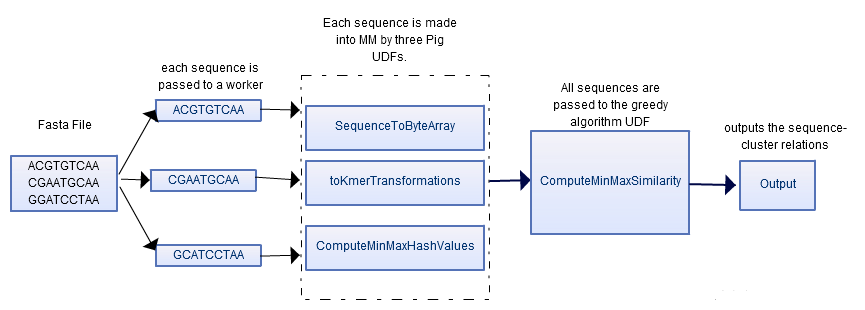
\includegraphics[scale=0.5]{data/MapReduce}
\caption{The flow of the MapReduce FrameWork using Pig}\label{fig:mapredflow}
\end{figure}

The Pig Script used to create this flow for the {\bf MM} algorithm can be seen in Alg. \ref{alg:pigscript}. Line 1 loads all the sequences from the file. Then, in line 2 the sequences are converted to bytes, which facilitates the conversion of the $k$-mer. The \$PROGRAM variable defines whether the input is DNA or RNA. In line 3, all files that contained an unknown character are sorted out. Line 4 produces the $k$-mer transformations for $k$-mer size \$KMER\_SIZE. The {\bf MM} sketch is then produced in line 5, using \$HASH\_SIZE hash functions. Line 6 and 7 are used to count the number of sequences to cluster. Finally, line 8 takes all sequences in to run the Greedy Clustering on them. $\epsilon$ is given by \$THRESHOLD. In line 8 MapReduce is not applied, as it runs the function on all sequences at once. So, the advantage of MapReduce over a non-parallel solution will only affect line 1 through 7.
\begin{algorithm}
\caption{Pig Script for MapReduce {\bf MM} Greedy Cluster Algorithm}\label{alg:pigscript}
\textbf{Input:} a list of DNA/RNA sequences $S=\{s_0,s_1,...,s_{N-1}\}$ of length $N$.\\
\textbf{Parameters:} \$HASH\_SIZE number of hash functions, \$KMER\_SIZE size of $k$-mer,	\$THRESHOLD is $\epsilon$\\
\textbf{Output:} list of the cluster each sequence belongs to in \textbf{results}.
\begin{algorithmic}[1]
\State sequences = LOAD '\$INPUT' USING FastaReader AS (line: chararray);
\State converted = FOREACH sequences GENERATE SequenceToByteArray(line, \$PROGRAM);
\State NoN = FILTER converted BY byteSeq is not null;
\State kmers = FOREACH NoN GENERATE toKmerTransformations(byteSeq, \$KMER\_SIZE);
\State minmaxvalues = FOREACH kmers GENERATE FLATTEN (ComputeMaxMinHashValues (kmerlist, \$HASH\_SIZE, \$KMER\_SIZE));
\State grouped = GROUP minmaxvalues ALL;
\State a\_count = FOREACH grouped GENERATE COUNT (minmaxvalues);
\State results = FOREACH grouped GENERATE FLATTEN (ComputeMaxMinSimilarity (minmaxvalues, a\_count.\$0, \$HASH\_SIZE, \$THRESHOLD));
\end{algorithmic}
\end{algorithm}

\end{document}